\documentclass[tikz,border=12pt]{standalone}
\usepackage[T1]{fontenc}
\usepackage{mathpazo}
\usepackage{amsmath,amssymb}
\usetikzlibrary{arrows.meta, calc}

\definecolor{stblue}{HTML}{7B97AD}
\definecolor{rwgold}{HTML}{B8995E}
\definecolor{sage}{HTML}{7A9A7E}
\definecolor{dkbrown}{HTML}{3D3530}
\definecolor{wmgray}{HTML}{7B7067}
\definecolor{cream}{HTML}{F9F6F0}
\definecolor{border}{HTML}{D4C9B8}
\definecolor{terracotta}{HTML}{C47A6A}
\definecolor{lavender}{HTML}{907EA0}

\begin{document}
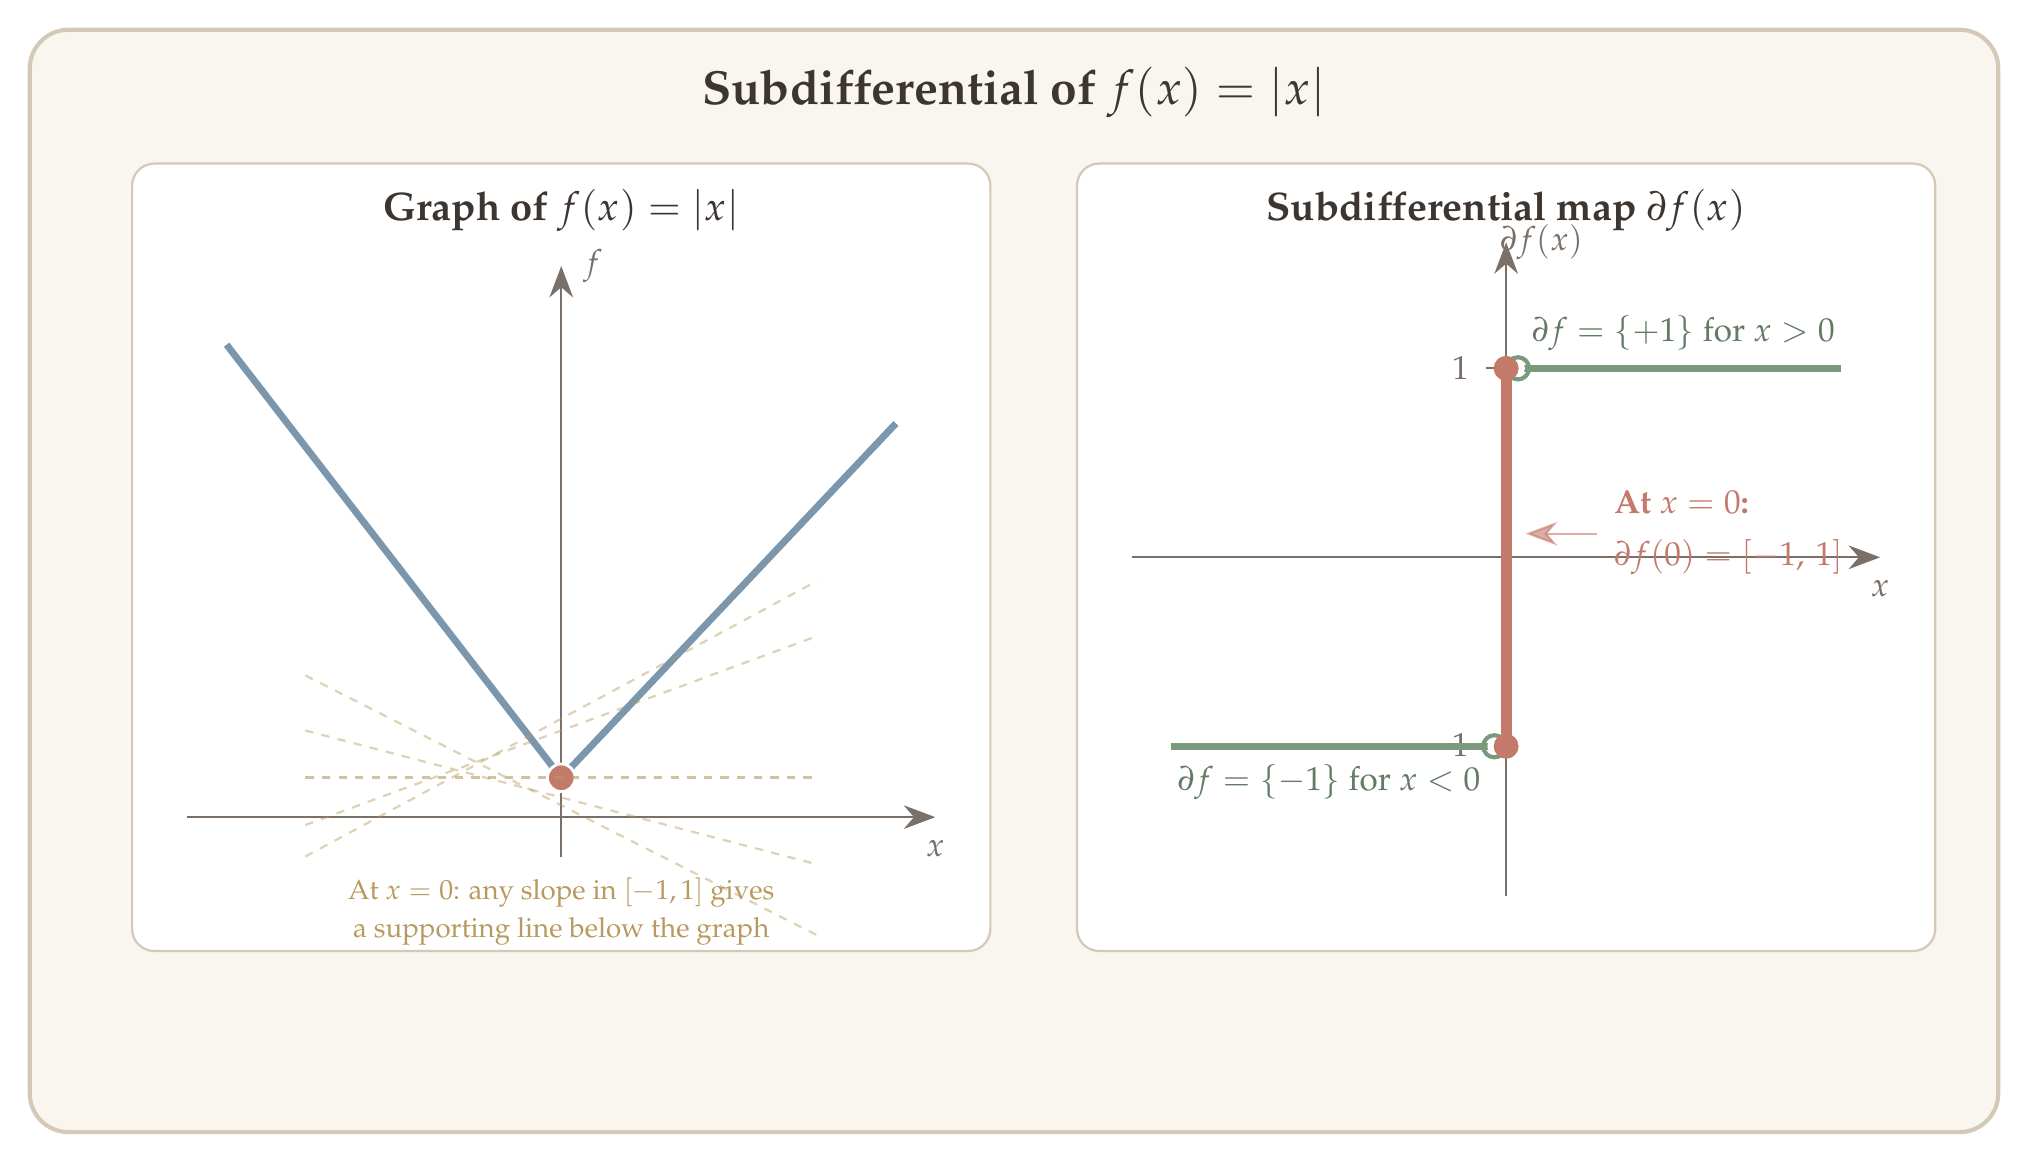
\begin{tikzpicture}[>={Stealth[length=4mm, width=3mm]}]

% Background — wider and taller for more breathing room
\fill[cream, rounded corners=14pt] (-1.0,-1.5) rectangle (24.0,12.5);
\draw[border, line width=1.5pt, rounded corners=14pt] (-1.0,-1.5) rectangle (24.0,12.5);

% Title
\node[text=dkbrown, font=\LARGE\bfseries] at (11.5,11.7) {Subdifferential of $f(x) = |x|$};

% ============================================================
% Left panel: graph of |x| with supporting lines
% ============================================================
\fill[white, rounded corners=8pt] (0.3,0.8) rectangle (11.2,10.8);
\draw[border, line width=0.8pt, rounded corners=8pt] (0.3,0.8) rectangle (11.2,10.8);
\node[text=dkbrown, font=\Large\bfseries] at (5.75,10.2) {Graph of $f(x) = |x|$};

% Axes — generous padding from panel edges
\draw[wmgray, line width=0.8pt, ->] (1.0,2.5) -- (10.5,2.5);
\draw[wmgray, line width=0.8pt, ->] (5.75,2.0) -- (5.75,9.5);
\node[text=wmgray, font=\large] at (10.5,2.1) {$x$};
\node[text=wmgray, font=\large] at (6.15,9.5) {$f$};

% |x| function — V shape, well within axes
\draw[stblue, line width=2.5pt] (1.5,8.5) -- (5.75,3.0) -- (10.0,7.5);

% Kink at origin
\fill[terracotta] (5.75,3.0) circle (5pt);
\draw[white, line width=1pt] (5.75,3.0) circle (5pt);

% Supporting lines at the kink (various slopes in [-1,1])
\draw[rwgold, line width=0.8pt, dashed, opacity=0.45] (2.5,2.0) -- (9.0,5.5);   % slope ~0.5
\draw[rwgold, line width=0.8pt, dashed, opacity=0.45] (2.5,2.4) -- (9.0,4.8);   % slope ~0.4
\draw[rwgold, line width=1pt, dashed, opacity=0.6]    (2.5,3.0) -- (9.0,3.0);   % slope 0
\draw[rwgold, line width=0.8pt, dashed, opacity=0.45] (2.5,3.6) -- (9.0,1.9);   % slope ~-0.3
\draw[rwgold, line width=0.8pt, dashed, opacity=0.45] (2.5,4.3) -- (9.0,1.0);   % slope ~-0.5

% Annotation below left panel
\node[text=rwgold, font=\normalsize, align=center] at (5.75,1.3)
  {At $x = 0$: any slope in $[-1,1]$ gives\\[2pt]
   a supporting line below the graph};

% ============================================================
% Right panel: subdifferential map (set-valued)
% ============================================================
\fill[white, rounded corners=8pt] (12.3,0.8) rectangle (23.2,10.8);
\draw[border, line width=0.8pt, rounded corners=8pt] (12.3,0.8) rectangle (23.2,10.8);
\node[text=dkbrown, font=\Large\bfseries] at (17.75,10.2) {Subdifferential map $\partial f(x)$};

% Axes
\draw[wmgray, line width=0.8pt, ->] (13.0,5.8) -- (22.5,5.8);
\draw[wmgray, line width=0.8pt, ->] (17.75,1.5) -- (17.75,9.8);
\node[text=wmgray, font=\large] at (22.5,5.4) {$x$};
\node[text=wmgray, font=\large] at (18.2,9.8) {$\partial f(x)$};

% Tick marks for +1 and -1
\draw[wmgray, line width=0.6pt] (17.5,8.2) -- (17.75,8.2);
\node[text=wmgray, font=\large, left] at (17.4,8.2) {$1$};
\draw[wmgray, line width=0.6pt] (17.5,3.4) -- (17.75,3.4);
\node[text=wmgray, font=\large, left] at (17.4,3.4) {$-1$};

% Right branch: +1 for x > 0
\draw[sage, line width=2.5pt] (17.9,8.2) -- (22.0,8.2);
\draw[sage, line width=1.5pt] (17.9,8.2) circle (4pt);
\fill[white] (17.9,8.2) circle (2.5pt);
\node[text=sage!80!black, font=\large, above=3pt] at (20.0,8.2) {$\partial f = \{+1\}$ for $x > 0$};

% Left branch: -1 for x < 0
\draw[sage, line width=2.5pt] (13.5,3.4) -- (17.6,3.4);
\draw[sage, line width=1.5pt] (17.6,3.4) circle (4pt);
\fill[white] (17.6,3.4) circle (2.5pt);
\node[text=sage!80!black, font=\large, below=3pt] at (15.5,3.4) {$\partial f = \{-1\}$ for $x < 0$};

% At x=0: vertical interval [-1, 1]
\draw[terracotta, line width=4pt, line cap=round] (17.75,3.4) -- (17.75,8.2);
\fill[terracotta] (17.75,3.4) circle (4.5pt);
\fill[terracotta] (17.75,8.2) circle (4.5pt);

% Annotation for x=0 — placed to the right, away from the vertical bar
\node[text=terracotta, font=\large\bfseries, align=left, anchor=west] at (19.0,6.5)
  {At $x = 0$:};
\node[text=terracotta, font=\large, align=left, anchor=west] at (19.0,5.8)
  {$\partial f(0) = [-1,\, 1]$};

% Small arrow pointing from annotation to the vertical bar
\draw[terracotta, line width=0.8pt, ->, opacity=0.6] (18.9,6.1) -- (18.0,6.1);

\end{tikzpicture}
\end{document}
